% Eight-slide research narrative. All numerical results come from reviewed bundles.
% See README.md for the slide-to-source map. No simulations run during compilation.
\documentclass[aspectratio=169,11pt]{beamer}
\usepackage{fontspec}
\setsansfont{texgyreheros-regular.otf}[
  BoldFont=texgyreheros-bold.otf,
  ItalicFont=texgyreheros-italic.otf,
  BoldItalicFont=texgyreheros-bolditalic.otf]
\usepackage{amsmath,booktabs,array,tikz,pgfplots}
% Slightly larger 16:9 canvas keeps tables and evidence footers comfortably spaced.
\geometry{paperwidth=192mm,paperheight=108mm}
\pgfplotsset{compat=1.18}
\definecolor{ink}{HTML}{152D42}
\definecolor{teal}{HTML}{008C95}
\definecolor{blue}{HTML}{2864DC}
\definecolor{orange}{HTML}{D46732}
\definecolor{muted}{HTML}{637487}
\definecolor{pale}{HTML}{EDF4F7}
\definecolor{gold}{HTML}{DBB465}
\setbeamercolor{normal text}{fg=ink,bg=white}
\setbeamercolor{structure}{fg=teal}
\setbeamercolor{frametitle}{fg=ink}
\setbeamercolor{block title}{fg=teal,bg=pale}
\setbeamercolor{block body}{fg=ink,bg=pale}
\setbeamerfont{frametitle}{size=\Large,series=\bfseries}
\setbeamersize{text margin left=8mm,text margin right=8mm}
\setbeamertemplate{navigation symbols}{}
\setbeamertemplate{frametitle}{\vspace{3mm}\insertframetitle\par\vspace{1mm}}
\setbeamertemplate{footline}{%
  \hspace{8mm}\textcolor{muted}{\scriptsize Gabriel Berezovsky\quad /\quad VO\textsubscript{2} simulation study}
  \hfill\textcolor{teal}{\scriptsize\insertframenumber\,/\,8}\hspace{8mm}\vspace{3mm}
}
\newcommand{\eyebrow}[1]{{\color{teal}\scriptsize\bfseries\MakeUppercase{#1}}\par\vspace{2mm}}
\newcommand{\takeaway}[1]{\par\vspace{2mm}\begin{beamercolorbox}[sep=2mm,wd=\linewidth]{block body}\small\bfseries #1\end{beamercolorbox}}
\newcommand{\src}[1]{\par\vfill{\fontsize{6.5}{8}\selectfont\color{muted}Evidence: #1. Full run IDs and metric definitions in the accompanying README.\par}}
\newcommand{\key}[2]{\par{\color{teal}\Large\bfseries #1}\par\small #2\par}
\pgfplotsset{journey/.style={
  axis line style={muted!60},tick style={muted!50},
  tick label style={font=\scriptsize,color=muted},
  label style={font=\small,color=ink},
  grid=major,grid style={pale},axis on top,
  legend style={draw=none,fill=none,font=\scriptsize},
  every axis plot/.append style={line width=1pt},
}}
\hypersetup{pdftitle={VO2 Simulations: From Working Oscillator to Experimental Fit},pdfauthor={Gabriel Berezovsky}}

\begin{document}

% 1. A title slide that also defines the scientific target.
\begin{frame}[t]
\eyebrow{Research progress / 15 September 2026}
{\fontsize{27}{32}\selectfont\bfseries VO\textsubscript{2} simulations:\\
from working oscillator\\to experimental fit\par}
\vspace{3mm}
{\color{muted}\normalsize Supporting automatic gain control in transimpedance amplifiers\par}
\vspace{4mm}
{\normalsize Gabriel Berezovsky\par}
{\small Supervised by Amir Gildor and Prof. Yoav Kalcheim\par}
\vspace{4mm}
\begin{columns}[T,onlytextwidth]
\begin{column}{.31\textwidth}\key{22 traces}{Measured current waveforms\\drive the simulations.}\end{column}
\begin{column}{.31\textwidth}\key{11 oscillators}{Match which records oscillate,\\and which remain stable.}\end{column}
\begin{column}{.33\textwidth}\key{One parameter set}{Match voltage level, amplitude,\\frequency and persistence.}\end{column}
\end{columns}
\takeaway{Our goal is quantitative agreement across currents, not simply a waveform that oscillates.}
\end{frame}

% 2. Separate the mechanism control from specimen calibration.
\begin{frame}[t]{First: establish the mechanism, then calibrate the sample}
\eyebrow{Foundation / August 2026}
\begin{columns}[T,onlytextwidth]
\begin{column}{.47\textwidth}
\textbf{Yuanhang-based control}\par\vspace{2mm}
\small Could the current-driven implementation sustain cycles without reaching zero volts?
\vspace{2mm}
\begin{block}{What we changed}
\small At $600\,\mu$A, increased $C_{\rm th}$ fourfold:\\
$49.63\rightarrow198.51$ pJ/K.\\
Other parameters retained Yuanhang's values.
\end{block}
\small Result: stable cycles at $0.222$ MHz;\\
steady voltage range $0.906$--$6.333$ V.\par
\vspace{2mm}
\small\textcolor{teal}{$V_{\rm floor}\approx I R_m$}: metallic resistance sets the steady floor; $C$ changes the approach.
\end{column}
\begin{column}{.49\textwidth}
\textbf{Replace control values with sample evidence}\par\vspace{2mm}
\small
\renewcommand{\arraystretch}{1.32}
\begin{tabular}{@{}ll@{}}
\toprule
Input & Adopted value / basis\\\midrule
$R(T)$ & Fit the measured major loop\\
$R_m$ & $18.22\,\Omega$\\
$T_0$ & $314.4$ K\\
$S_e$ & $3.675\,\mu$W/K, from $P/\Delta T$\\
$C$ & $0.39$ pF, timing upper bound\\
$C_{\rm th}$ & $0.04787$ pJ/K, from $S_e\tau_{\rm th}$\\
$\gamma$ & $0.95627$, initially borrowed\\\bottomrule
\end{tabular}\par
\vspace{1mm}
\scriptsize Thermal estimates depend on static $R(T)$ and circuit interpretation. The major loop does not identify $\gamma$.
\end{column}
\end{columns}
\takeaway{A working control verifies the mechanism; it is not a fit to our specimen.}
\src{control 6765e0; resistance 0849a9; thermal estimates 761640 and aa2469; report Sections 1--6}
\end{frame}

% 3. Compare objective values only within the same objective definition.
\begin{frame}[t]{Trial 1: better waveform error did not recover oscillations}
\eyebrow{Frozen prediction $\rightarrow$ constrained fit $\rightarrow$ relaxed fit / 29 August}
\small We replayed the measured current inputs. Then we fitted eight shared parameters\\
using waveform, mean, amplitude, spectrum, frequency and edge errors.
\vspace{3mm}
\renewcommand{\arraystretch}{1.45}
\begin{tabular}{@{}p{3.1cm}p{4.8cm}rr@{}}
\toprule
\textbf{Run} & \textbf{What changed} & \textbf{All-trace $J\!\downarrow$} & \textbf{Oscillating}\\\midrule
Frozen estimates & No waveform tuning & 0.8813 & 0 / 22\\
Constrained search & Stay inside supported intervals & 0.8750 & 0 / 22\\
Relaxed diagnostic & Expand bounds; remove prior & 0.6827 & 0 / 22\\\bottomrule
\end{tabular}\par
\vspace{3mm}
\begin{columns}[T,onlytextwidth]
\begin{column}{.47\textwidth}
\key{0.67 mV}{Frozen-model mean-voltage error at the stable $189.6\,\mu$A record. Static agreement was good.}
\end{column}
\begin{column}{.49\textwidth}
\key{22.5\% lower error}{Relaxed fit improved $J$, but 7 of 8 parameters left their supported intervals. Only transients remained.}
\end{column}
\end{columns}
\takeaway{Reducing waveform error can reward a good average or a large transient, without producing sustained cycles.}
\src{frozen eefab7; global fit 8f12d6; 17 training and 5 initially held-out records; final evaluation 0.05 ns}
\end{frame}

% 4. Preserve the historical label metric, explicitly distinguish it from persistence.
\begin{frame}[t]{Trials 2--4: trading oscillation detection against amplitude}
\eyebrow{Change the objective, then constrain the physics / 29 August -- 7 September}
\small We successively emphasized oscillation detection, voltage amplitude, and independently supported parameters.
\vspace{3mm}
\renewcommand{\arraystretch}{1.38}
\begin{tabular}{@{}p{3.6cm}p{6.0cm}rr@{}}
\toprule
\textbf{Run} & \textbf{Search strategy} & \textbf{Labels$^{*}$} & \textbf{Amplitude MAE}\\\midrule
Oscillation-priority & Reward detection; relax bounds & 21 / 22 & 289.6 mV\\
Amplitude-priority & Increase amplitude penalty & 19 / 22 & 81.2 mV\\
Physics-anchored & Anchor six supported parameters & 22 / 22 & 212.5 mV\\\bottomrule
\end{tabular}\par
\vspace{2mm}
{\scriptsize\color{muted}$^{*}$Historical peak-count labels, not persistence. Amplitude MAE uses the same 11 experimental oscillators in every row.\par}
\vspace{3mm}
\begin{columns}[T,onlytextwidth]
\begin{column}{.47\textwidth}
\textbf{What improved}\par\small
We could generate cycles across many currents. Amplitude weighting reduced voltage excursions; anchoring limited parameter drift.
\end{column}
\begin{column}{.49\textwidth}
\textbf{What remained unrealistic}\par\small
The anchored fit needed $C=6.84$ pF, about $17.5\times$ the timing bound, and $\gamma=0.157$. Median amplitude was still $5.55\times$ measured.
\end{column}
\end{columns}
\takeaway{Each strategy improved a different target. None established a physically supported, quantitative fit.}
\src{ac1c5e at 0.05 ns; 85526c and 717797 at 0.025 ns; objective values are not directly comparable across searches}
\end{frame}

% 5. Lossless plotted samples from the reviewed audit, not graph digitization.
\begin{frame}[t]{The turning point: some ``oscillations'' were dying out}
\eyebrow{Persistence audit / 14 September}
\begin{columns}[T,onlytextwidth]
\begin{column}{.64\textwidth}
\begin{tikzpicture}
\begin{axis}[journey,width=\linewidth,height=4.6cm,xmin=50,xmax=250,ymin=80,ymax=205,
 xlabel={Time (ns)},ylabel={Voltage (mV)},
 title={\small $606\,\mu$A: same measured current input},
 legend style={at={(.5,-.28)},anchor=north,legend columns=2}]
\addplot[blue] table[x=time_ns,y=experiment,col sep=comma]{data/current_606uA.csv};
\addlegendentry{Experiment}
\addplot[orange] table[x=time_ns,y=reference,col sep=comma]{data/current_606uA.csv};
\addlegendentry{Anchored model}
\end{axis}
\end{tikzpicture}
\end{column}
\begin{column}{.32\textwidth}
\textbf{What we now measure}\par\vspace{2mm}
\small Four consecutive 50 ns windows: amplitude, mean, frequency and decay.
\vspace{3mm}
\key{$50.2\rightarrow0.49$ mV}{Model raw peak-to-peak span, first to last window at 0.025 ns.}
\vspace{2mm}
\small Experiment stays near $10$--$12$ mV. The plotted fine-step replay shows the same failure.
\end{column}
\end{columns}
\vspace{4mm}
\takeaway{At the finest step, the previous fit sustains only 9 of the 11 measured oscillators. The old 22/22 claim was too permissive.}
\src{audit 26ff13; plot at 0.00625 ns; operational persistence thresholds, with sensitivity checks, are documented in report Section 11}
\end{frame}

% 6. Feature metrics here use a different, explicitly stated late-time window.
\begin{frame}[t]{Trial 5: controlled parameter maps exposed the trade-off}
\eyebrow{126 shared combinations / 228, 381 and 606 $\mu$A}
\small Vary $C$, $\tau_{\rm th}=C_{\rm th}/S_e$ and $\gamma$; hold other parameters at the anchored fit.\\
Balance amplitude, frequency, mean voltage and decay. Recheck selected points on all 22 records.
\vspace{3mm}
\renewcommand{\arraystretch}{1.3}
\begin{tabular}{@{}p{4cm}rrrp{5.1cm}@{}}
\toprule
\textbf{Selected point} & \textbf{$C$ (pF)} & \textbf{Recovered / 11} & \textbf{False +} & \textbf{Remaining failure}\\\midrule
Best feature match & 8.0 & 10 & 0 & High-current cycles decay\\
Best persistent point & 8.0 & 11 & 1 & Amplitude far too large\\
Best within timing bound & 0 & 0 & 0 & No sustained cycles\\\bottomrule
\end{tabular}\par
\vspace{3mm}
\begin{columns}[T,onlytextwidth]
\begin{column}{.47\textwidth}
\key{$294.5$ vs $9.25$ mV}{Persistent-point vs measured late amplitude at $606\,\mu$A: $31.8\times$ too large.}
\end{column}
\begin{column}{.49\textwidth}
\key{No shared fit}{No mapped point with $C\leq0.39$ pF sustains cycles at any of the three selected currents.}
\end{column}
\end{columns}
\takeaway{Preserving cycles is not enough: the same parameters must also match their size and the non-oscillating records.}
\src{26ff13; table at 0.00625 ns; amplitude = 5--95\% span over 150--250 ns; grid slices are not an exhaustive search}
\end{frame}

% 7. Compact table makes conditional-vs-measured quantities explicit.
\begin{frame}[t]{Trial 6: test the resistance law without another optimizer}
\eyebrow{Conditional reconstruction from measured power / 14 September}
\small Infer a thermal history from measured current and voltage, then replay the hysteresis law:
\vspace{-1mm}
\[
I_R=I-C\dot V,\quad R_{\rm eff}=V/I_R,\quad
C_{\rm th}\dot T=VI_R-S_e(T-T_0).
\]
\vspace{-2mm}
\begin{columns}[T,onlytextwidth]
\begin{column}{.65\textwidth}
\renewcommand{\arraystretch}{1.3}
\begin{tabular}{@{}rrrr@{}}
\toprule
\textbf{Current ($\mu$A)} & \textbf{Inferred $T$ (K)} & \textbf{Measured $R_{\rm eff}$ ($\Omega$)} & \textbf{Replayed $R$ ($\Omega$)}\\\midrule
189.6 & 330.91 & 1680.6 & 1679.2\\
228.7 & 328.96 & 1017.9 & 1762.5\\
381.1 & 333.64 & 488.4 & 1215.1\\
606.7 & 344.25 & 298.2 & 29.7\\\bottomrule
\end{tabular}\par
\end{column}
\begin{column}{.32\textwidth}
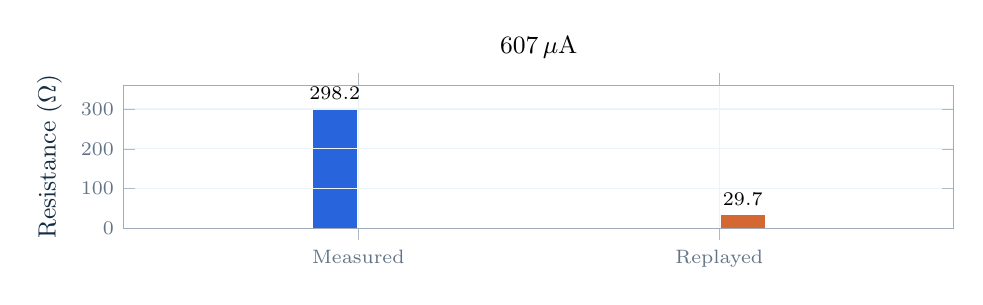
\begin{tikzpicture}
\begin{axis}[journey,width=\linewidth,height=3.4cm,
 ymin=0,ymax=360,xmin=-.65,xmax=1.65,
 xtick={0,1},xticklabels={Measured,Replayed},ytick={0,100,200,300},
 title={\small $607\,\mu$A},ylabel={Resistance ($\Omega$)},
 ybar,bar width=15pt,enlarge x limits=false,
 nodes near coords,nodes near coords style={font=\scriptsize},
 grid=major]
\addplot[fill=blue,draw=blue] coordinates {(0,298.2)};
\addplot[fill=orange,draw=orange] coordinates {(1,29.7)};
\end{axis}
\end{tikzpicture}
\end{column}
\end{columns}
\vspace{3mm}
\small At $607\,\mu$A, four tested $\gamma$ values give only \textbf{26--34 $\Omega$}.\\
Even the upper $S_e$ bound gives \textbf{71--112 $\Omega$}, still below $298\,\Omega$.
\takeaway{Changing $\gamma$ alone did not close the gap. The inconsistency involves the resistance law, thermal assumptions or channel interpretation.}
\src{fa4b66; means over 150--250 ns; central $C=0.39$ pF and $\gamma=0.95627$. Temperature is conditional, not independently measured; below-onset agreement is not independent validation}
\end{frame}

% 8. Close with conclusions, not an unqualified claim of model failure.
\begin{frame}[t]{What we learned -- and the next decisive test}
\eyebrow{Conclusion / No new calibrated parameter set adopted}
\begin{columns}[T,onlytextwidth]
\begin{column}{.47\textwidth}
\textbf{Established by these trials}\par\vspace{3mm}
\small
\textcolor{teal}{01}\quad A working oscillator is not a sample fit.\par\vspace{3mm}
\textcolor{teal}{02}\quad Lower error and correct peak labels can conceal incorrect dynamics.\par\vspace{3mm}
\textcolor{teal}{03}\quad We have not found a shared, physically supported fit to amplitude, frequency and persistence.
\end{column}
\begin{column}{.49\textwidth}
\textbf{Next: verify the measurement-to-model map}\par\vspace{3mm}
\small Identify where voltage was measured and how current was reconstructed.\par\vspace{3mm}
Establish whether $V/I$ is device resistance or includes contacts, load or readout response.\par\vspace{3mm}
Then test one explicit correction at a time; validate on currents not used to tune it.
\end{column}
\end{columns}
\vspace{3mm}
\takeaway{The next gain should come from testing an assumption, not merely increasing the optimizer budget.}
\vspace{2mm}
\small\color{muted}Possible missing ingredients: dynamic or partial switching, nonuniform heating, or the actual TIA circuit. These remain hypotheses, not demonstrated causes.
\src{reviewed evidence through 14 September; all runs, source data and reproduction commands remain archived}
\end{frame}

\end{document}
